\section{Practice}
\label{sec:experiments}

This section will provide the implementation details of the theory part (section \ref{sec:theory}). The algorithm is implemented in C ++ and makes use of the CGAL library (\url{https://www.cgal.org}). Then, given the implementation, some preliminary experimental setup will be introduced. The experimental setup will include different types of test polygons and observations of the algorithm performance.
% As such, we will devise an algorithm for optimising the positions of the guards inside the given Art Gallery polygon. 
% The algorithm is coded in C ++ with the use of the CGAL library (\url{https://www.cgal.org}).
\subsection{Implementation}
In section \ref{sec:theory} we devised formula \ref{eq:l} for computing the gradient of one guard and the reflex vertices it can see. This section will thus show the implementation and use of the formula to iteratively optimise a guard's position. 

The implementation takes a polygon and a guard with an arbitrary position as input. The main idea of the algorithm is that the position of the guard is continuously improved until an optimum is found. That is, until the computed gradient does not change the position of the guard anymore.
It can happen that the gradient computes an optimised position of the guard outside the polygon. In that case, the guard is placed and subsequently moved on the polygon boundary. The pseudo-code can be found in Algorithm \ref{alg:1g}.

\begin{algorithm}[H]
    \begin{algorithmic}[1]
    \caption{Position Optimisation for One Guard}
    \label{alg:1g}

    \State{\textbf{Input:} polygon $\mathcal P$, guard $p(x, y)$}
    \State{\textbf{Output:} optimised position $p'(x', y')$ of the guard}
    \State{}
    % \For{\textbf{each} guard $p(x, y)$}
    \State{\textit{cur\_guard\_position} $\gets p(x, y)$}

    \While{\textit{prev\_guard\_position} $\neq$ \textit{cur\_guard\_position}} %\Comment{continue as long as there are no more improvements in the guard's position}
        % \State{compute \textit{visibility\_region} of $p$}
        \State{compute $\bigtriangledown f(\textit{cur\_guard\_position})$}
        \State{\textit{prev\_guard\_position} $\gets$ \textit{cur\_guard\_position}}
        \State{\textit{cur\_guard\_position} $\gets \textit{prev\_guard\_position} + l\bigtriangledown f$}

        \If{\textit{cur\_guard\_position} is outside the polygon}
            \State{place \textit{cur\_guard\_position} on polygon boundary}
        \EndIf
    \EndWhile
    \State{$p'(x', y') \gets \textit{cur\_guard\_position}$}
    % \EndFor
    \State \Return $p'$
    \end{algorithmic}
\end{algorithm}

The implementation has been tested with one guard and multiple input polygons. The polygons target specific use- or edge-cases. These cases will be built upon when expanding the implementation to multiple guards. The input polygons are:

% are the irrational guard polygon (Figure \ref{fig:p}), a star-shaped polygon (Subfigure \ref{fig:star}), a comb-shaped polygon (Subfigure \ref{fig:comb}), an arrow head (Subfigure \ref{fig:concave}) and an arbitrary polygon (Subfigure \ref{fig:random}). Each of them will be used for testing various aspects of the algorithm as follows:

\begin{itemize}
    \item the \textbf{star polygon} (Subfigure \ref{fig:star}) tests whether guards can do basic moves from the inside the polygon to the centre of it. The star polygon can be fully seen by 1 guard.
    \item the \textbf{arrowhead polygon} (Subfigure \ref{fig:concave}) tests the movement of guard to optimality on the boundary of the polygon. The arrowhead polygon can be fully seen by 1 guard.
    \item the \textbf{comb polygon} (Subfigure \ref{fig:comb}) tests the algorithm with multiple guards. The comb polygon can be fully guarded by 4 points, each of them placed in each one of the spikes.
    \item the \textbf{arbitrary polygon} (Subfigure \ref{fig:random}) combines the previously mentioned cases. The arbitrary polygon can be fully seen by 3 guards.
    \item the \textbf{irrational guards polygon} (Figure \ref{fig:p}) combines the previously mentioned cases. The irrational guards polygon can be fully seen by either 3 guards with irrational coordinates, or 4 guards with rational coordinates.
\end{itemize}

\begin{figure}[h!]
    \centering
    \begin{subfigure}{0.45\textwidth}
        \centering
        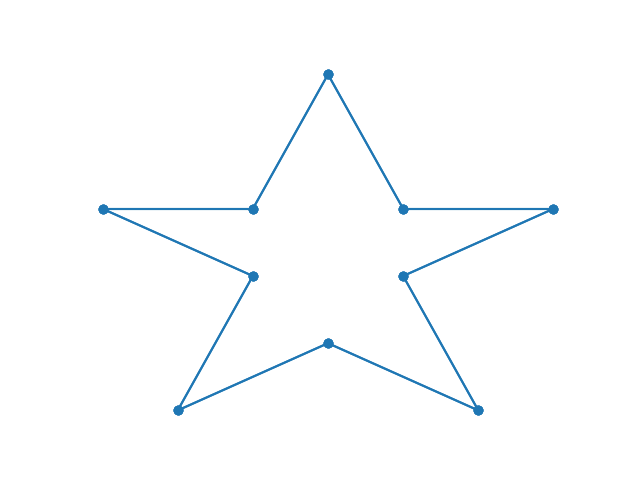
\includegraphics[width = \textwidth]{pentagram.png}
        \caption{Star test input polygon.}
        \label{fig:star}
    \end{subfigure}
    \begin{subfigure}{0.45\textwidth}
        \centering
        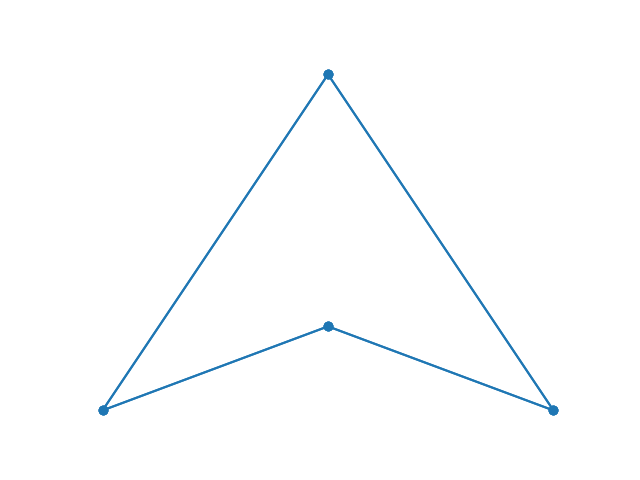
\includegraphics[width = \textwidth]{concave_triangle.png}
        \caption{Arrowhead test input polygon.}
        \label{fig:concave}
    \end{subfigure}
    \begin{subfigure}{0.45\textwidth}
        \centering
        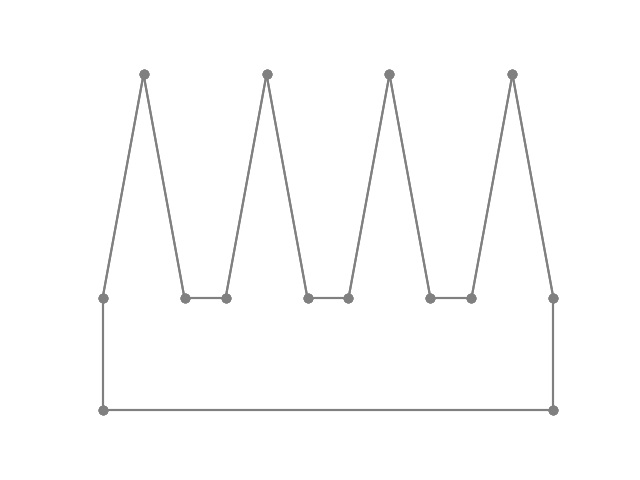
\includegraphics[width = \textwidth]{comb.png}
        \caption{Comb test input polygon.}
        \label{fig:comb}
    \end{subfigure}
    \begin{subfigure}{0.45\textwidth}
        \centering
        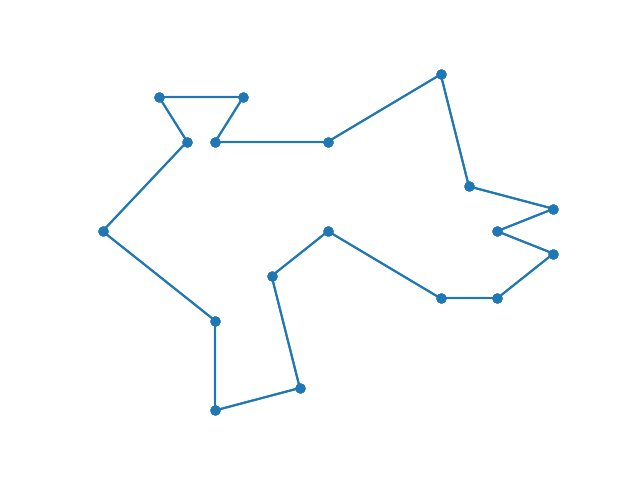
\includegraphics[width = \textwidth]{random.png}
        \caption{Arbitrary test input polygon.}
        \label{fig:random}
    \end{subfigure}
    \caption{Input polygons used for testing the algorithm.}
\end{figure}
% Timetable and planning What will you do with the remainder of my thesis? Give an approximate estimation/timetable for what you will do and when you will be done.
\subsection{Preliminary Results}
The implementation was tested on the five previously mentioned input polygons and an arbitrarily placed guard. The gradient descent was computed with a learning rate of 0.2. The choice behind the learning rate is that it is big enough to find an optimum position in a reasonable runtime. It is also small enough to observe a smooth, relevant transition in the guard's position.

The experiments had a 1-minute run timeout. This amount of time was chosen in order to build some intuition related to the speed of the algorithm. Namely, we expect that the algorithm would be fast for small input polygons. That is the case with the star and the arrowhead polygons in Subfigures \ref{fig:star_gradient} and \ref{fig:concave_gradient}. There, the final guard positions are optimally found within 1 minute. From this position, the polygons are fully seen.


\begin{figure}[h!]
    \centering
    \begin{subfigure}{0.45\textwidth}
        \centering
        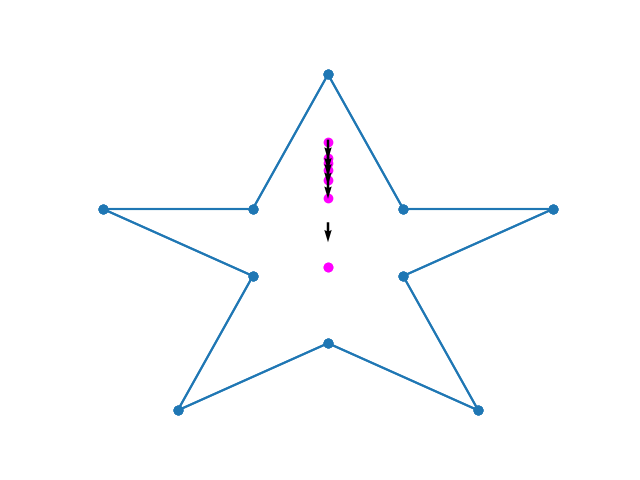
\includegraphics[width = \textwidth]{pentagram_gradient.png}
        \caption{Star polygon gradient example}
        \label{fig:star_gradient}
    \end{subfigure}
    \begin{subfigure}{0.45\textwidth}
        \centering
        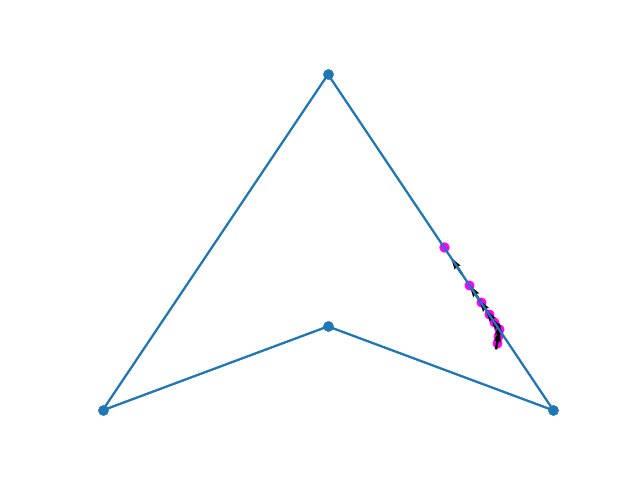
\includegraphics[width = \textwidth]{concave_triangle_gradient.png}
        \caption{Arrowhead polygon gradient example.}
        \label{fig:concave_gradient}
    \end{subfigure}
    \begin{subfigure}{0.45\textwidth}
        \centering
        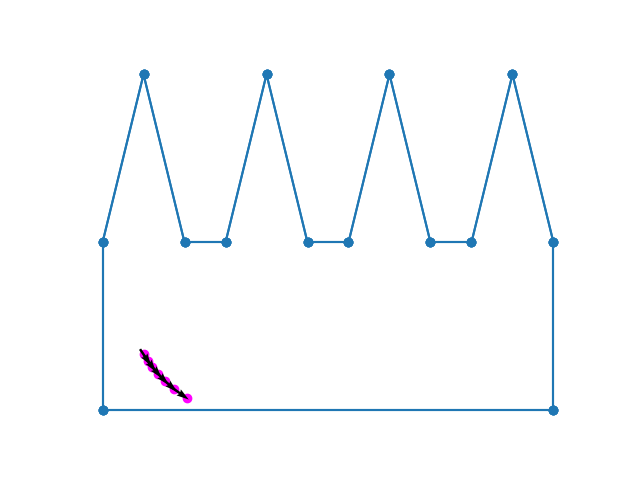
\includegraphics[width = \textwidth]{comb_gradient.png}
        \caption{Comb polygon gradient example.}
        \label{fig:comb_gradient}
    \end{subfigure}
    \begin{subfigure}{0.45\textwidth}
        \centering
        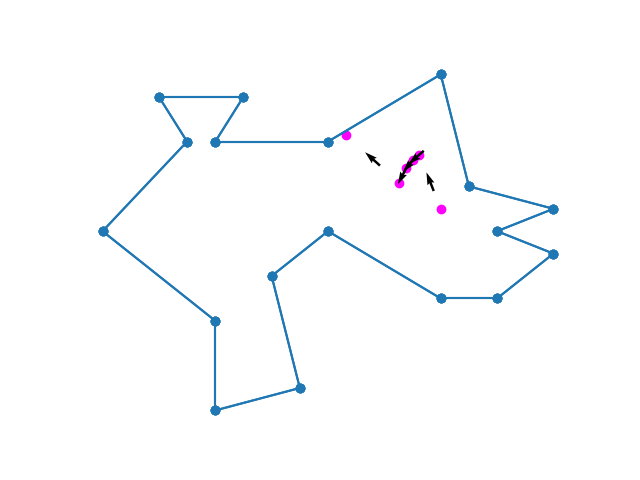
\includegraphics[width = \textwidth]{random_gradient.png}
        \caption{Arbitrary polygon gradient example.}
        \label{fig:random_gradient}
    \end{subfigure}
    \begin{subfigure}{\textwidth}
        \centering
        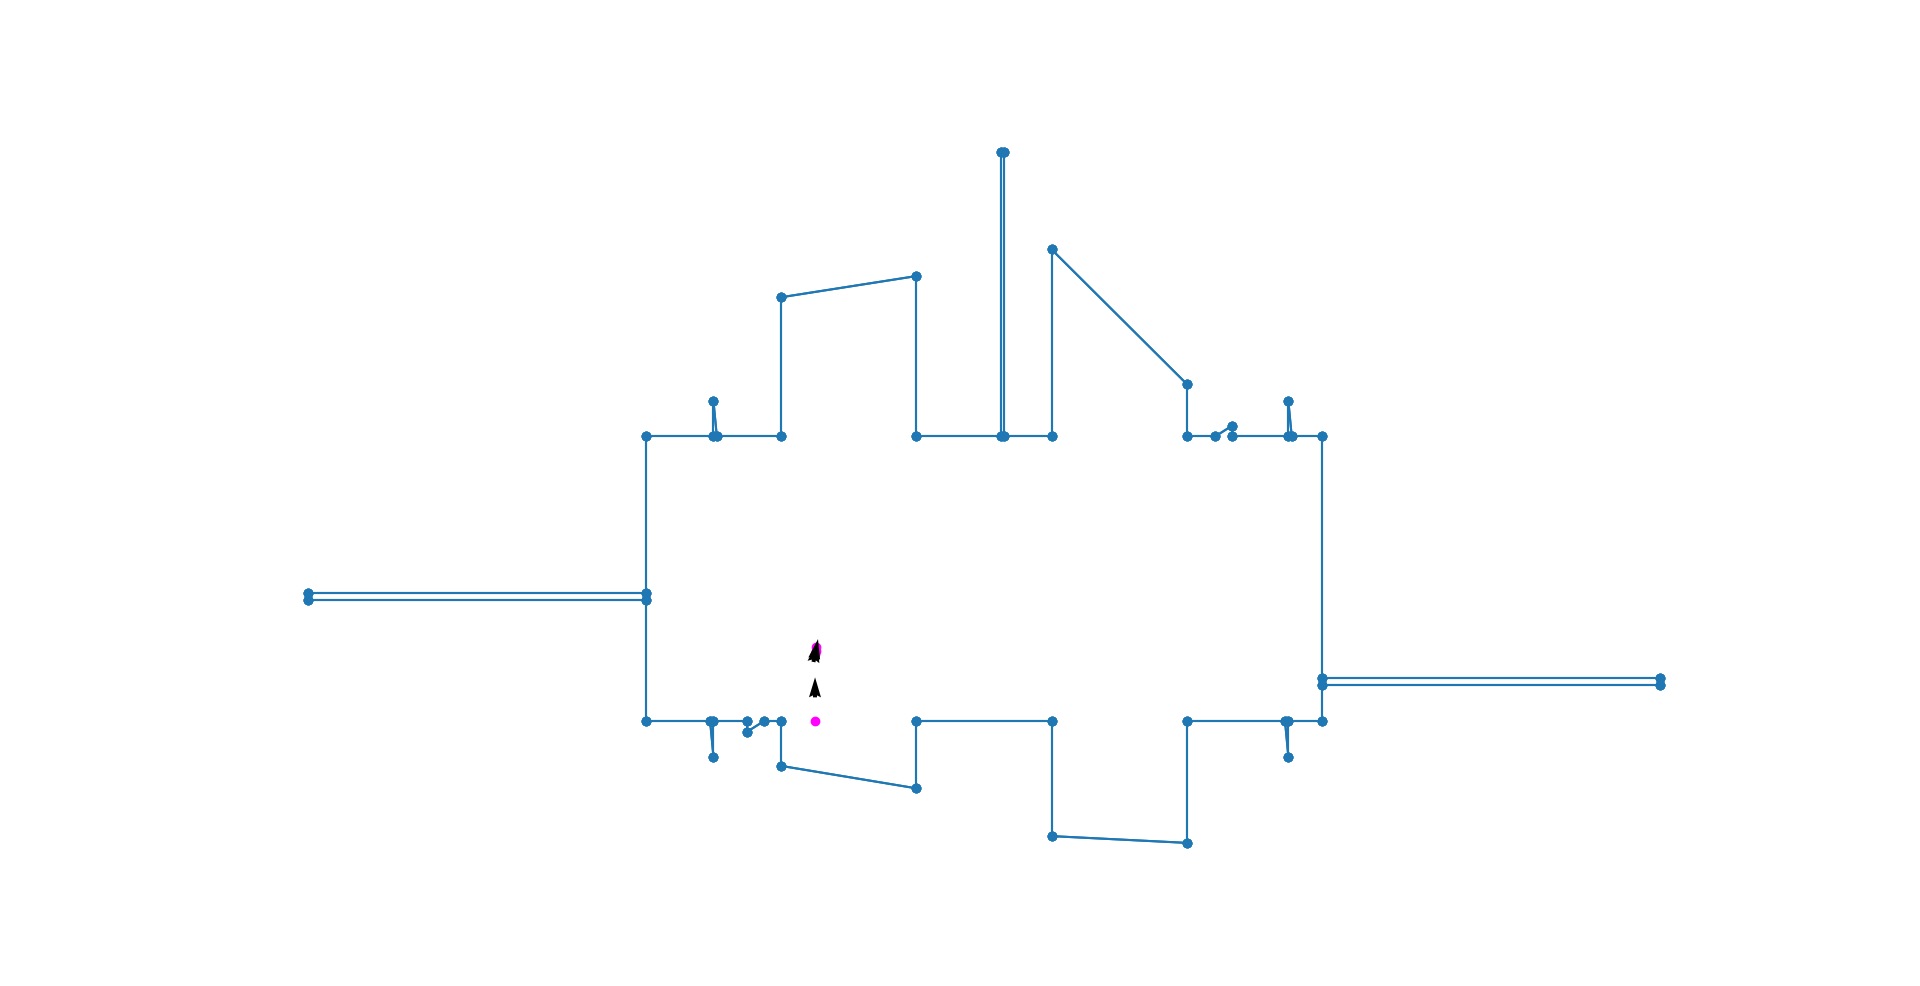
\includegraphics[width = \textwidth]{love_gradient.png}
        \caption{Arbitrary polygon gradient example.}
        \label{fig:love_gradient}
    \end{subfigure}
    \caption{Gradient descent examples with learning rate $l = 0.2$ on the test polygons.}
    \label{fig:gradients}
\end{figure}

This is not the case with the rest of the three input polygons. The final position of the guard in Subfigures \ref{fig:comb_gradient}, \ref{fig:random_gradient} and \ref{fig:love_gradient} is the last computed position at timeout. Additionally, all of these polygons require multiple guards to be fully visible. For this reason, we expect that gradient descent would either settle in a local optimum, or would continuously jump between multiple local optima given a large enough learning rate.

In the case of the comb (Subfigure \ref{fig:comb_gradient}), the tendency of the guard is to move towards the lower boundary of the polygon. This maximises the area observed by the guard, even though the guard is not able to see all the spikes at once. When given a longer timeout, we expect that the algorithm would move the guard between the local optima below each of the spikes.

The arbitrary polygon (Subfigure \ref{fig:random_gradient}) shows similar behaviour in terms of moving between local optima. Initially the guard takes a large jump from its initial position to a more fine-tuned path. After a few smoother steps, it takes another large jump close to the boundary of the polygon. Nonetheless, this polygon cannot be fully guarded by 1 point. In order to explore this aspect, we will later look into how the jumps between local optima differ given the learning rate.

Lastly, the algorithm managed to take the least number of steps within the time limit (slowest) in the irrational guard polygon (Subfigure \ref{fig:love_gradient}). That is expected, as it is also the largest polygon out of all the input ones. This polygon can also not be guarded by only 1 point. So, later in this paper we will also explore how the algorithm performs when different learning rates are used. 
% Moreover, we will also examine how well our approximation gradient descent algorithm performs when compared to the exact irrational positions of the guards.


% \newpage
\subsubsection{Different Learning Rates}
We also experimented with how increasing the learning rate would affect the outcome of the algorithm on the test polygons. Namely, we tested how increasing the learning rate from $l = 0.2$ to $l \in \{0.4, 0.65\}$ would affect the one-guard placement in the input polygons. As such, we chose the arrowhead and the arbitrary polygons as the two test cases. This is due to the fact that the former polygon requires only one guard for full visibility, while the latter requires more. Figure \ref{fig:multiple_gradients} displays some preliminary results for exploring this aspect. 

Subfigures \ref{fig:concave_gradient_045} and \ref{fig:concave_gradient_06} show the transition from $l = 0.45$ to $l = 0.6$, respectively, for the arrowhead polygon. As expected, the steps between the guard positions are bigger. Since only one guard is required to fully view the polygon, the optimum is clearly achieved in both cases. The only major difference between the two learning rates is that when $l$ is larger, less steps are needed to reach the optimum, as our intuition predicts.

\begin{figure}[h!]
    \centering
    \begin{subfigure}{0.45\textwidth}
        \centering
        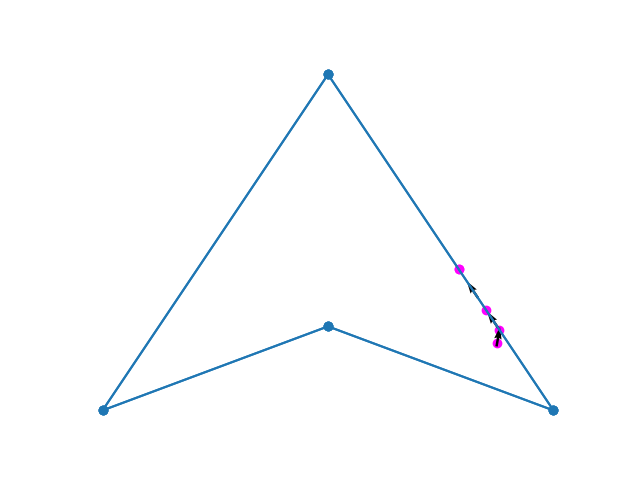
\includegraphics[width = \textwidth]{concave_triangle_gradient_045.png}
        \caption{Arrowhead polygon gradient with learning rate $l = 0.45$ example}
        \label{fig:concave_gradient_045}
    \end{subfigure}
    \begin{subfigure}{0.45\textwidth}
        \centering
        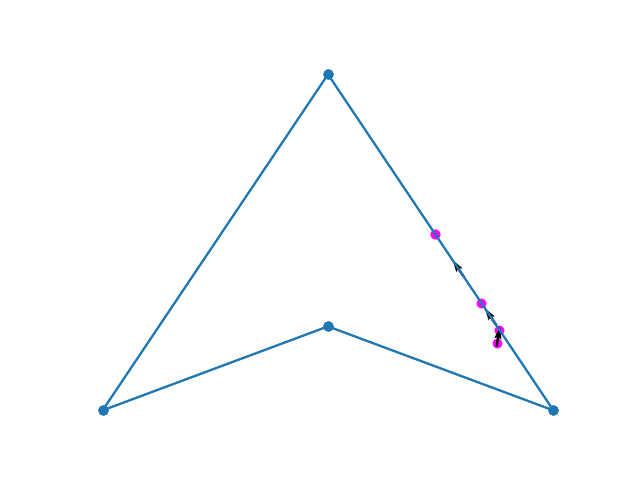
\includegraphics[width = \textwidth]{concave_triangle_gradient_06.png}
        \caption{Arrowhead polygon gradient with learning rate $l = 0.6$ example.}
        \label{fig:concave_gradient_06}
    \end{subfigure}
    \begin{subfigure}{0.45\textwidth}
        \centering
        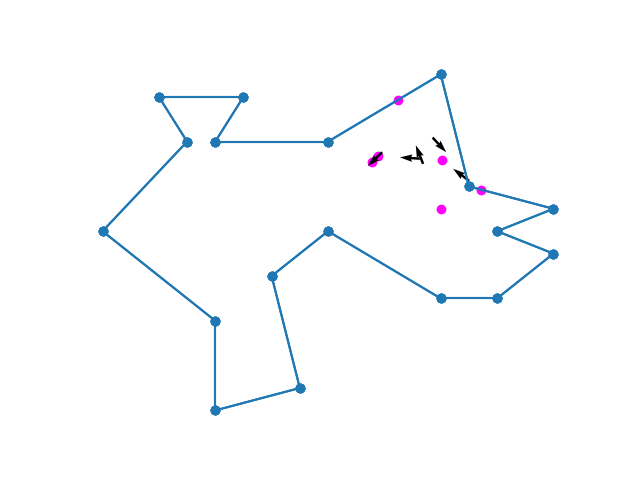
\includegraphics[width = \textwidth]{random_gradient_045.png}
        \caption{Arbitrary polygon gradient with learning rate $l = 0.45$ example.}
        \label{fig:random_gradient_045}
    \end{subfigure}
    \begin{subfigure}{0.45\textwidth}
        \centering
        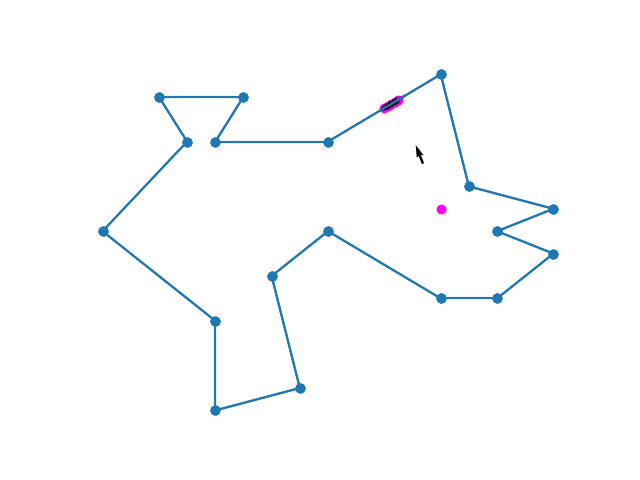
\includegraphics[width = \textwidth]{random_gradient_06.png}
        \caption{Arbitrary polygon gradient with learning rate $l = 0.6$ example.}
        \label{fig:random_gradient_06}
    \end{subfigure}
    \caption{Gradient descent examples with learning rate $l \in \{0.45, 0.6\}$ on the one-guard Arrowhead and multiple guards arbitrary input polygons.}
    \label{fig:multiple_gradients}
\end{figure}

Subfigures \ref{fig:random_gradient_045} and \ref{fig:random_gradient_06} show the transition for the arbitrary polygon from $l = 0.45$ to $l = 0.6$, respectively. Unlike the arrowhead polygon, the arbitrary polygon appears to show a complete opposite evolution. When $l = 0.45$, the guard does not follow a clear path towards an optimum. Instead, it appears that after a few steps it returns to a position close to the starting position. This type of cycling could be accounted for by the gradient computation being unable to escape a local optimum. When $l = 0.6$, we would expect that the guard path is even more chaotic and dispersed. However, the learning rate in this case turns out to be large enough to escape the local optimum that $l = 0.45$ was stuck in. Nonetheless, we expect that even with a larger learning rate, the guard path would still not reach an optimum final position. Because the arbitrary polygon requires multiple guards for full visibility, we predict that the one guard would still be stuck in a cycle between all the guards' local optima.

Therefore, we predict that the choice of the learning rate will be closely intertwined with the type of input polygon and the number of guards required to guard it. This situation will be considered more in-depth in the later phases of this thesis. Then, we can assess whether this is the case given a gradient computation algorithm for multiple guards.